\section*{Parte 2}\label{sec:parte2}
\subsection*{Criação do Schema}

Uma vez recolhidos os dados, foi necessário guardar os mesmos de forma organizada em estruturas independentes daquelas já existentes na base de dados Oracle. Para tal procedemos à criação do tablespace, datafile e utilizador que permitiram que tal aconteça.

\subsection*{Tablespace e Datafile}
 
Antes de ser feito o armazenamento de dados na base de dados, foi criado em primeiro lugar um \textit{tablespace} permanente, \textbf{assignment\_tables}, que conterá todos os objetos do utilizador  da nossa BD, armazenados fisicamente no \textit{datafile} \textbf{assignment\_tables\_1}:

\begin{verbatim}
CREATE TABLESPACE assignment_tables
    DATAFILE '\u01\app\oracle\oradata\orcl12\orcl\assignment_tables_1.dbf'
        SIZE 200M;
\end{verbatim}
  
Em seguida, foi criado o \textit{tablespace} temporário, onde são armazenados os dados temporários de uma determinada sessão por um determinado período de tempo. Este \textit{tablespace} possui um \textit{tempfile} e, não um \textit{datafile}, e é utilizado quando um utilizador, ao qual o tablespace temporário foi atribuído, inicia operações. Sendo assim, o tablespace temporário armazena os dados temporários utilizados em transações de utilizadores:

\begin{verbatim}
CREATE TEMPORARY TABLESPACE assignment_temp
    TEMPFILE '\u01\app\oracle\oradata\orcl12\orcl\assignment_temp_1.dbf'
        SIZE 50M
        AUTOEXTEND ON;
\end{verbatim}

\subsection*{User e Grants}

Uma vez criados os \textit{tablespaces} e \textit{datafiles}, foi criada a conta do utilizador através da qual é feito o login à base de dados. Para criar o utilizador foi especificado que os objetos por ele criados ficariam armazenados no \textit{tablespace}  referido anteriormente:

\begin{verbatim}
CREATE USER mic
    IDENTIFIED BY oracle
    DEFAULT TABLESPACE assignment_tables
    TEMPORARY TABLESPACE assignment_temp;

\end{verbatim}


O privilégio CREATE SESSION garante que o utilizador criado se consiga conectar à base de dados, e com os restantes privilégios concedidos este pode criar e manipular os objetos da BD:

\begin{verbatim}
GRANT CREATE SESSION TO mic;
GRANT CREATE TABLE TO mic;
GRANT CREATE VIEW TO mic;
GRANT CREATE ANY TRIGGER TO mic;
GRANT CREATE ANY PROCEDURE TO mic;
GRANT CREATE SEQUENCE TO mic;
GRANT CREATE SYNONYM TO mic;
\end{verbatim}

Por defeito, ao ser criado o utilizador não tem quota no tablespace, sendo necessária a sua atribuição para que este possa criar objetos:
\begin{verbatim}
ALTER USER mic QUOTA 200M ON assignment_tables;
\end{verbatim}

Depois de ser estabelecida uma ligação à base de dados com este utilizador, foram criadas as tabelas e procedimentos necessários para armazenar de forma correta os dados, como veremos na secção seguinte.

\subsection*{Tabelas}
De forma a poder guardar os dados inicialmente recolhidos, foi necessária a criação de tabelas para esse efeito. Tendo em conta que para a monitorização da base de dados seria necessário atualizar  constantemente os dados recolhidos e guardar toda a informação que a cada momento é consultada, para algumas das tabelas criadas foi também gerada uma tabela de "histórico", isto é, uma tabela que para uma determinada instância de dados vai guardar as mudanças relativas a esses dados. Para permitir registar estas mudanças, foi necessário associar aos dados recolhidos um \textit{timestamp}. Mais à frente são explicadas com mais detalhe as tabelas de histórico

Em seguida é apresentada para cada tabela a DDL para a sua geração, bem como uma breve explicação dos atributos e chaves que compõe a tabela.
\subsubsection*{Tablespaces}

A tabela \textbf{tablespaces} armazena todos os dados recolhidos considerados relevantes em relação aos \textit{tablespaces} da base de dados Oracle, o que incluí o seu nome, o espaço utilizado, o espaço livre, o espaço total e a percentagem de espaço utilizado.

A chave primária desta tabela é o nome do tablespace visto ser o único atributo que identifica univocamente uma instância da entidade:

\begin{verbatim}
CREATE TABLE tablespaces
    (   tablespace_name varchar2(50) not null,
        used_MB number not null,
        free_MB number not null,
        total_MB number not null,
        percentage_used number not null,
        timestamp timestamp not null,
        CONSTRAINT tablespaces_pk PRIMARY KEY (tablespace_name)
    );
    

\end{verbatim}
\subsubsection*{Datafiles}

A tabela \textbf{datafiles} armazena, tal como o nome indica, os dados recolhidos relativamente aos \textit{datafiles} do sistema. Estes são o identificador do datafile (file\_id), o nome do datafile, o nome do tablespace a que este está associado, o seu tamanho totalm o tamanho utilizado, o tamanho livre, e a percentagem de tamanho utilizado.

A chave primária desta tabela é o file\_id do datafile, por ser o atributo de menor tamanho e o único que identfica unicamente uma instância desta tabela.

 A tabela \textbf{datafiles} tem uma chave estrangeira, tablespace\_name, que faz referência à chave primária da tabela \textbf{tablespaces}. Cada \textit{tablespace} numa base de dados Oracle consiste em um ou mais \textit{datafiles}, o que justifica a existência deste relacionamento:



\begin{verbatim}
CREATE TABLE datafiles
    (   file_id number not null,
        datafile_name varchar2(512) not null,
        tablespace_name varchar2(50) not null,
        total_MB number not null,
        used_MB number not null,
        free_MB number not null,
        percentage_used number not null,
        timestamp timestamp not null,
        CONSTRAINT datafiles_pk PRIMARY KEY(file_id),
        CONSTRAINT fk_tablespaces FOREIGN KEY(tablespace_name)
            REFERENCES tablespaces(tablespace_name)
    );
\end{verbatim}
\subsubsection*{Users}

Na tabela \textbf{users} são armazenados os dados recolhidos relativamente aos utilizadores da base de dados Oracle, nomeadamente o user identificador, o nome, o tablespace permanente a que estão associados, assim como o temporário, o estado da conta do utilizador, a quota no tablespace, os privilégios que lhe foram concedidos e a sua utiliação de cpu.

A chave primária de \textbf{users} é o user\_id, por ser o único atributo que identifica univocamente um utilizador.

Esta tabela tem uma chave estrangeira, default\_tablespaces, que faz referência à chave primária da tabela \textbf{tablespaces}, ou seja ao nome do tablespace:
\begin{verbatim}

CREATE TABLE users
    (   user_id number not null,
        name varchar2(50) not null,
        default_tablespace varchar2(50) not null,
        temporary_tablespace varchar2(50) not null,
        account_status varchar2(20) not null,
        quota number not null,
        privilege varchar2(50),
        cpu_usage number,
        timestamp timestamp not null,
        CONSTRAINT users_pk PRIMARY KEY(user_id),
        CONSTRAINT fk_tablespaces_users FOREIGN KEY(default_tablespace)
            REFERENCES tablespaces(tablespace_name)
    );
\end{verbatim}
\subsubsection*{Tables}

Nesta tabela armazenam-se todas as informações relativas às tabelas da base de dados, nomeadamente o nome do dono (utilizador) da tabela, o id desse utilizador, o nome da tabela, o nome do \textit{tablespace} onde a tabela foi criada, o número de acessos à tabela e o número de registos da mesma.

A chave primária desta de \textbf{tables} é composta pelo nome da tabela e o identificador do utilizador que a criou, uma vez que esta á única forma de identificar unicamente uma instância de \textbf{tables}. Diferentes utilizadores podem ter tabelas com o mesmo nome, e daí o nome da tabela não ser suficiente para constituir a chave primária. Desta composição justifica-se a existência da chave estrangeira owner\_id, que faz referência à chave primária da tabela \textbf{users}, ou seja o identificador do utiizador.



\begin{verbatim}
CREATE TABLE tables
    (   owner_name varchar2(30) not null,
        owner_id number not null,
        name varchar2(30) not null,
        correspondent_tablespace varchar2(50),
        nr_of_accesses number not null,
        nr_of_regists number not null,
        dropped varchar2(20) not null,
        timestamp timestamp not null,
        CONSTRAINT tables_pk PRIMARY KEY(owner_id,name),
        CONSTRAINT fk_users_tables FOREIGN KEY(owner_id)
            REFERENCES users(user_id)        
    );
\end{verbatim}
\subsubsection*{Memory}

Os dados recolhidos relativamente à memória do sistema são guardados na tabela \textbf{memory}, e consistem na memória utilizada, na memória livre e na percentagem de memória livre.

A chave primária desta tabela é o timestamp, que a cada momento da recolha de informação permite identificar univocamente o estado da memória:
\begin{verbatim}
CREATE TABLE memory
    (   total_size_bytes number not null,
        free_size_bytes number not null,
        percentage_free number not null,
        timestamp timestamp not null,
        CONSTRAINT memory_pk PRIMARY KEY (timestamp)
    );
\end{verbatim}
\subsubsection*{Sessions}

Os dados referentes às sessões na base de dados encontram-se armazenados na tabela \textbf{sessions}. É guardada informação relativamente ao id da sessão, ao nome do utilizador associado à sessão, o id associado a esse utilizador, o nome do \textit{schema} da sessão, e há quanto tempo a sessão foi iniciada.

A chave primária desta tabela é composta pelo id da sessão (session\_id) e o timestamp em que a informação sobre as sessões foi recolhida.

\textbf{Sessions} tem uma chave estrangeira, \textbf{user\_id}, que faz referência à chave primária da tabela \textbf{users}, isto é ao id do utilizador, uma vez que um utilizador pode ter uma ou mais sessões ativas.

\begin{verbatim}
CREATE TABLE sessions
    (   session_id number not null,
        username varchar2(50) not null,
        user_id number not null,
        schema_name varchar2(50) not null,
        login_time varchar2(50) not null,
        timestamp timestamp not null,
        CONSTRAINT sessions_pk PRIMARY KEY (session_id,timestamp),
        CONSTRAINT fk_users FOREIGN KEY (user_id)
            REFERENCES users(user_id)
        
    );
\end{verbatim}
\subsubsection*{Io\_reads}

A tabela \textbf{io\_reads} armazena a informação relativa às leituras ao disco, que consiste no nome da métrica, o tempo de início da leitura, o tempo final da leitura e o valor da métrica.

A chave primária de \textbf{io\_reads} é o timestamp visto ser o único atributo que identifica univocamente uma instância desta tabela.
\begin{verbatim}
    
CREATE TABLE io_reads
    (
    metric_name varchar2(64) not null,
    begin_time timestamp not null,
    end_time timestamp not null,
    value number not null,
    timestamp timestamp not null,
    CONSTRAINT io_reads_pk PRIMARY KEY (timestamp)
    );
\end{verbatim}
\subsubsection*{Io\_writes}
A tabela \textbf{io\_writes} armazena a informação relativa às escritas ao disco, que consiste no nome da métrica, o tempo de início da leitura, o tempo final da leitura e o valor da métrica.

A chave primária de \textbf{io\_writes} é o timestamp, que tal como para a tabela \textbf{io\_reads}, é o único atributo que identifica univocamente uma instância desta tabela.
\begin{verbatim}
CREATE TABLE io_writes
    (
    metric_name varchar2(64) not null,
    begin_time timestamp not null,
    end_time timestamp not null,
    value number not null,
    timestamp timestamp not null,
    CONSTRAINT io_writes_pk PRIMARY KEY (timestamp)
    );
    
\end{verbatim}
\subsection*{Histórico e Triggers}
Como referido anteriormente, para algumas das tabelas foi necessário criar uma tabela de histórico para guardar registo das mudanças aos dados, de cada vez que são atualizados. A tabela de histórico é também útil para manter as tabelas "ativas" na base de dados, ou seja com a informação mais recente, com um tamanho consideravelmente reduzido. As tabelas \textbf{tablespaces}, \textbf{datafiles}, \textbf{users}, \textbf{tables} e \textbf{sessions} têm uma tabela de histórico associada, cuja única diferença em relação à tabela "mãe" é a de a chave primária ser composta também pelo timestamp.

Para guardar as mudanças  foi criado um\textit{trigger} que é acionado sempre que há atualização dos dados na tabela a que a tabela de histórico se refere. A título de exemplo, é mostrada a tabela de histórico e trigger para inserção da dados na tabela \textbf{tablespaceshistory}, que se refere aos dados da tabela \textbf{tablespaces}:
\\


\begin{verbatim}
CREATE TABLE tablespaceshistory
    (   tablespace_name varchar2(50) not null,
        used_MB number not null,
        free_MB number not null,
        total_MB number not null,
        percentage_used number not null,
        timestamp timestamp not null,
        CONSTRAINT tablespaceshistory_pk PRIMARY KEY (tablespace_name,timestamp)

\end{verbatim}
O \textit{trigger} é do tipo AFTER INSERT, e quando é feita um \textit{update} na tabela \textbf{tablespaces}, pega nos valores que estavam na tabela e insere-os na tabela de histórico:
\begin{verbatim}
CREATE OR REPLACE TRIGGER insert_into_tablespaceshistory
AFTER UPDATE ON tablespaces FOR EACH ROW
BEGIN
    INSERT INTO tablespaceshistory
        (tablespace_name,used_MB,free_MB,total_MB,percentage_used,timestamp)
    VALUES
        (:OLD.tablespace_name,:OLD.used_MB,:OLD.free_MB,:OLD.total_MB,:OLD.percentage_used,:OLD.timestamp);   
END insert_into_tablespaceshistory;
/
\end{verbatim}





\newpage
\subsection*{Modelo Relacional}

\begin{figure}[h!]
 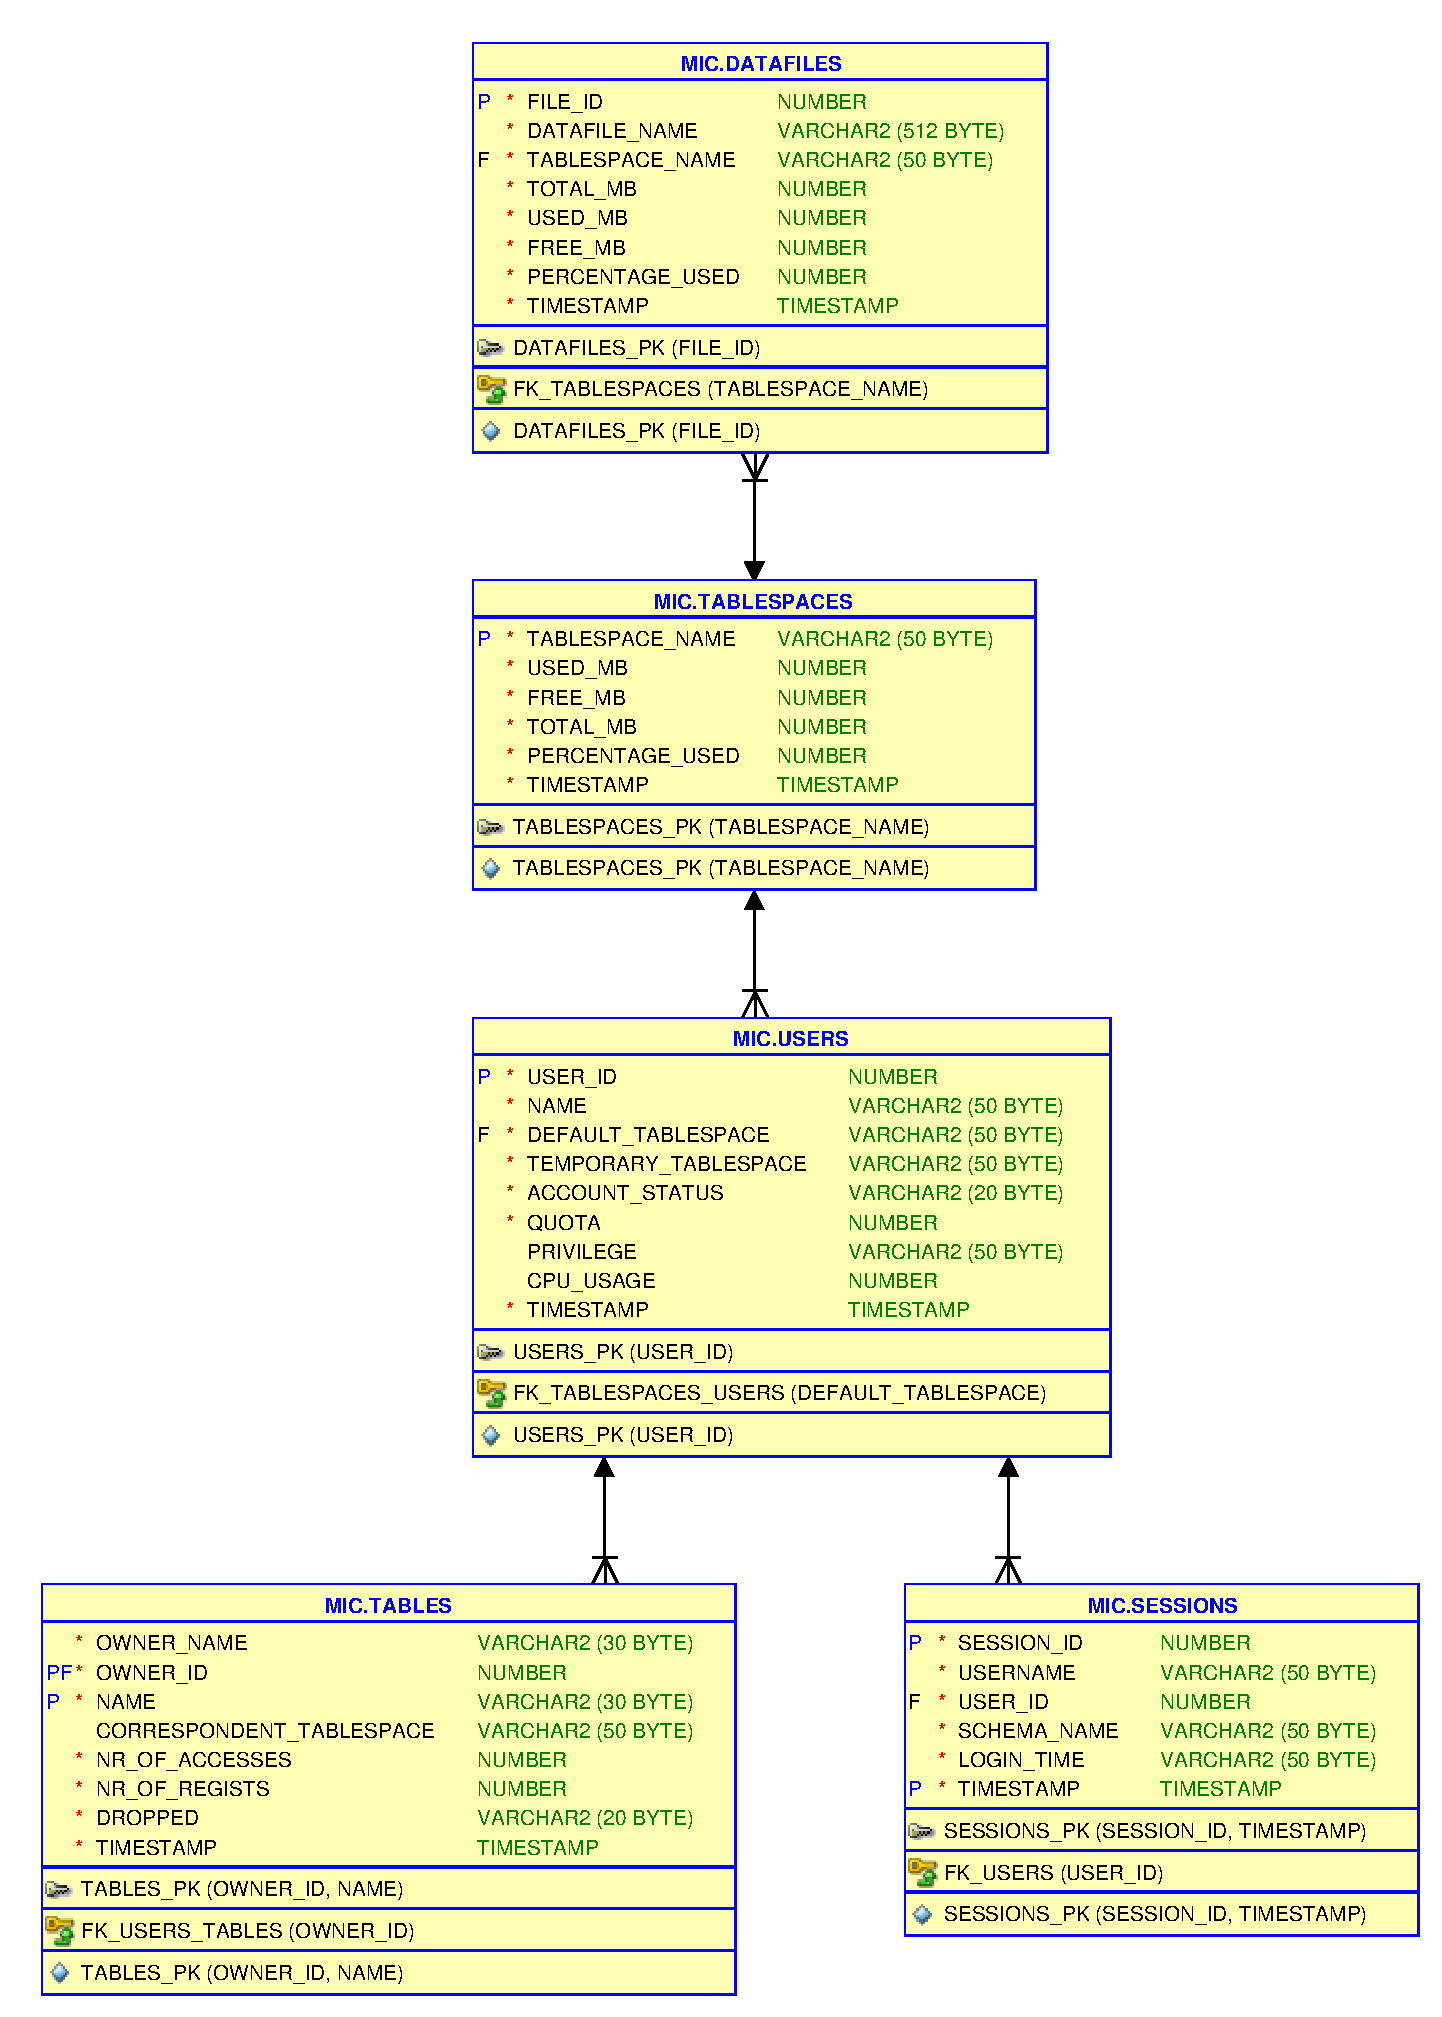
\includegraphics[scale=0.5]{tex/img/modelo_concetual.pdf}
    \caption{Modelo relacional da base de dados.} 
    \label{fig:modelo}
\end{figure}


